% =====================================================================
%  MSc Research Project - IEEE-style single-column report (NCI structure)
%  Navaneetha Thalakokkula (23213914) - MSc Cloud Computing, NCI
%  HOW TO USE: create a Blank Project in Overleaf, delete main.tex content,
%  paste this whole file, set Compiler = pdfLaTeX, click Recompile 2-3 times
%  (citations resolve after BibTeX runs). refs.bib is embedded below.
% =====================================================================
\documentclass[12pt,a4paper]{article}
\usepackage[utf8]{inputenc}
\usepackage[T1]{fontenc}
\usepackage{mathptmx}   % Times New Roman font (matches NCI sample papers)
\usepackage[margin=1in]{geometry}
\usepackage{graphicx}
\usepackage{booktabs}
\usepackage{amsmath,amssymb}
\usepackage{caption}
\usepackage{float}
\usepackage{cite}
\usepackage[hidelinks]{hyperref}
\usepackage{tikz}
\usetikzlibrary{shapes.geometric, arrows.meta, positioning, calc}
\usepackage{array}
\usepackage{multirow}

% ---- embedded bibliography: 31 entries, every DOI resolved against Crossref before use ----
\begin{filecontents*}{refs.bib}
@article{mirjalili2016whale,author={Mirjalili, Seyedali and Lewis, Andrew},title={The Whale Optimization Algorithm},journal={Advances in Engineering Software},year={2016},volume={95},pages={51--67},doi={10.1016/j.advengsoft.2016.01.008}}
@article{mirjalili2014grey,author={Mirjalili, Seyedali and Mirjalili, Seyed Mohammad and Lewis, Andrew},title={Grey Wolf Optimizer},journal={Advances in Engineering Software},year={2014},volume={69},pages={46--61},doi={10.1016/j.advengsoft.2013.12.007}}
@inproceedings{kennedy1995particle,author={Kennedy, James and Eberhart, Russell},title={Particle swarm optimization},booktitle={Proceedings of ICNN'95 -- International Conference on Neural Networks},year={1995},volume={4},pages={1942--1948},doi={10.1109/ICNN.1995.488968}}
@article{storn1997differential,author={Storn, Rainer and Price, Kenneth},title={Differential evolution -- a simple and efficient heuristic for global optimization over continuous spaces},journal={Journal of Global Optimization},year={1997},volume={11},number={4},pages={341--359},doi={10.1023/A:1008202821328}}
@article{heidari2019harris,author={Heidari, Ali Asghar and Mirjalili, Seyedali and Faris, Hossam and Aljarah, Ibrahim and Mafarja, Majdi and Chen, Huiling},title={Harris hawks optimization: Algorithm and applications},journal={Future Generation Computer Systems},year={2019},volume={97},pages={849--872},doi={10.1016/j.future.2019.02.028}}
@article{vanthieu2023mealpy,author={Van Thieu, Nguyen and Mirjalili, Seyedali},title={MEALPY: An open-source library for latest meta-heuristic algorithms in Python},journal={Journal of Systems Architecture},year={2023},volume={139},pages={102871},doi={10.1016/j.sysarc.2023.102871}}
@article{hochreiter1997long,author={Hochreiter, Sepp and Schmidhuber, J{\"u}rgen},title={Long short-term memory},journal={Neural Computation},year={1997},volume={9},number={8},pages={1735--1780},doi={10.1162/neco.1997.9.8.1735}}
@inproceedings{cho2014learning,author={Cho, Kyunghyun and van Merri{\"e}nboer, Bart and Gulcehre, Caglar and Bahdanau, Dzmitry and Bougares, Fethi and Schwenk, Holger and Bengio, Yoshua},title={Learning phrase representations using RNN encoder--decoder for statistical machine translation},booktitle={Proceedings of the 2014 Conference on Empirical Methods in Natural Language Processing (EMNLP)},year={2014},pages={1724--1734},doi={10.3115/v1/D14-1179}}
@article{beloglazov2012optimal,author={Beloglazov, Anton and Buyya, Rajkumar},title={Optimal online deterministic algorithms and adaptive heuristics for energy and performance efficient dynamic consolidation of virtual machines in cloud data centers},journal={Concurrency and Computation: Practice and Experience},year={2012},volume={24},number={13},pages={1397--1420},doi={10.1002/cpe.1867}}
@techreport{reiss2011google,author={Reiss, Charles and Wilkes, John and Hellerstein, Joseph L.},title={Google cluster-usage traces: format + schema},institution={Google Inc.},address={Mountain View, CA, USA},year={2011},note={Revised 2014}}
@inproceedings{wiesner2021lets,author={Wiesner, Philipp and Behnke, Ilja and Scheinert, Dominik and Gontarska, Kordian and Thamsen, Lauritz},title={Let's wait awhile: How temporal workload shifting can reduce carbon emissions in the cloud},booktitle={Proceedings of the 22nd International Middleware Conference (Middleware '21)},year={2021},pages={260--272},doi={10.1145/3464298.3493399}}
@article{radovanovic2023carbon,author={Radovanovi{\'c}, Ana and Koningstein, Ross and Schneider, Ian and Chen, Bokan and Duarte, Alexandre and Roy, Binz and Xiao, Diyue and Haridasan, Maya and Hung, Patrick and Care, Nick and Talukdar, Saurav and Mullen, Eric and Smith, Kendal and Cottman, MariEllen and Cirne, Walfredo},title={Carbon-aware computing for datacenters},journal={IEEE Transactions on Power Systems},year={2023},volume={38},number={2},pages={1270--1280},doi={10.1109/TPWRS.2022.3173250}}
@inproceedings{maji2022carboncast,author={Maji, Diptyaroop and Shenoy, Prashant and Sitaraman, Ramesh K.},title={CarbonCast: Multi-day forecasting of grid carbon intensity},booktitle={Proceedings of the 9th ACM International Conference on Systems for Energy-Efficient Buildings, Cities, and Transportation (BuildSys '22)},year={2022},pages={198--207},doi={10.1145/3563357.3564079}}
@book{holland1992adaptation,author={Holland, John H.},title={Adaptation in Natural and Artificial Systems: An Introductory Analysis with Applications to Biology, Control, and Artificial Intelligence},publisher={MIT Press},address={Cambridge, MA},year={1992}}
@article{beloglazov2012energy,author={Beloglazov, Anton and Abawajy, Jemal and Buyya, Rajkumar},title={Energy-aware resource allocation heuristics for efficient management of data centers for cloud computing},journal={Future Generation Computer Systems},year={2012},volume={28},number={5},pages={755--768},doi={10.1016/j.future.2011.04.017}}
@inproceedings{goiri2011greenslot,author={Goiri, {\'I}{\~n}igo and Le, Kien and Haque, Md. E. and Beauchea, Ryan and Nguyen, Thu D. and Guitart, Jordi and Torres, Jordi and Bianchini, Ricardo},title={GreenSlot: Scheduling energy consumption in green datacenters},booktitle={Proceedings of the 2011 International Conference for High Performance Computing, Networking, Storage and Analysis (SC '11)},year={2011},pages={1--11},doi={10.1145/2063384.2063411}}
@inproceedings{dodge2022measuring,author={Dodge, Jesse and Prewitt, Taylor and Tachet des Combes, Remi and Odmark, Erika and Schwartz, Roy and Strubell, Emma and Luccioni, Alexandra Sasha and Smith, Noah A. and DeCario, Nicole and Buchanan, Will},title={Measuring the carbon intensity of AI in cloud instances},booktitle={Proceedings of the 2022 ACM Conference on Fairness, Accountability, and Transparency (FAccT '22)},year={2022},pages={1877--1894},doi={10.1145/3531146.3533234}}
@article{kalra2015review,author={Kalra, Mala and Singh, Sarbjeet},title={A review of metaheuristic scheduling techniques in cloud computing},journal={Egyptian Informatics Journal},year={2015},volume={16},number={3},pages={275--295},doi={10.1016/j.eij.2015.07.001}}
@article{leerbeck2020short,author={Leerbeck, Kenneth and Bacher, Peder and Junker, Rune Gr{\o}nborg and Goranovi{\'c}, Goran and Corradi, Olivier and Ebrahimy, Razgar and Tveit, Anna and Madsen, Henrik},title={Short-term forecasting of CO2 emission intensity in power grids by machine learning},journal={Applied Energy},year={2020},volume={277},pages={115527},doi={10.1016/j.apenergy.2020.115527}}
@article{abbasikhazaei2022energy,author={Abbasi-khazaei, Tahereh and Rezvani, Mohammad Hossein},title={Energy-aware and carbon-efficient VM placement optimization in cloud datacenters using evolutionary computing methods},journal={Soft Computing},year={2022},volume={26},number={19},pages={9287--9322},doi={10.1007/s00500-022-07245-y}}
@article{khodayarseresht2023energy,author={Khodayarseresht, Ehsan and Shameli-Sendi, Alireza and Fournier, Quentin and Dagenais, Michel},title={Energy and carbon-aware initial VM placement in geographically distributed cloud data centers},journal={Sustainable Computing: Informatics and Systems},year={2023},volume={38},pages={100888},doi={10.1016/j.suscom.2023.100888}}
@article{miao2024energy,author={Miao, Zicong and Liu, Lei},title={Energy and carbon-aware distributed machine learning tasks scheduling scheme for the multi-renewable energy-based edge-cloud continuum},journal={Science and Technology for Energy Transition},year={2024},volume={79},pages={82},doi={10.2516/stet/2024076}}
@article{danach2026carbon,author={Danach, Kassem},title={Carbon-aware scheduling in cloud computing operations: A multi-objective optimisation approach},journal={IET Smart Grid},year={2026},doi={10.1049/stg2.70056}}
@article{ruparel2026carbon,author={Ruparel, Shivam},title={Carbon-aware scheduling and distributionally robust optimization for cloud systems: forecasting, battery storage, and adaptive ambiguity refinement},journal={Journal of Cloud Computing},year={2026},volume={15},doi={10.1186/s13677-026-00904-7}}
@inproceedings{moore2025sustainable,author={Moore, Jacob},title={Sustainable carbon-aware and water-efficient LLM scheduling in geo-distributed cloud datacenters},booktitle={Proceedings of the Great Lakes Symposium on VLSI (GLSVLSI '25)},year={2025},doi={10.1145/3716368.3735301}}
@article{zhang2024ewoa,author={Zhang, Yanfeng and Wang, Jiawei},title={Enhanced Whale Optimization Algorithm for task scheduling in cloud computing environments},journal={Journal of Engineering and Applied Science},year={2024},volume={71},pages={121},doi={10.1186/s44147-024-00445-3}}
@article{feng2025gwo,author={Feng, Hao and Li, Haoyu and Liu, Yuming and Cao, Kun and Zhou, Xiumin},title={A novel virtual machine placement algorithm based on grey wolf optimization},journal={Journal of Cloud Computing},year={2025},volume={14},pages={7},doi={10.1186/s13677-025-00730-3}}
@article{madhusudhan2023hho,author={Madhusudhan, H. S. and Satish Kumar, T. and Gupta, Punit and McArdle, Gavin},title={A Harris Hawk Optimisation system for energy and resource efficient virtual machine placement in cloud data centers},journal={PLOS ONE},year={2023},volume={18},number={8},pages={e0289156},doi={10.1371/journal.pone.0289156}}
@article{kumar2023eeoa,author={Santhosh Kumar, M. and Karri, Ganesh Reddy},title={EEOA: Cost and energy efficient task scheduling in a cloud-fog framework},journal={Sensors},year={2023},volume={23},number={5},pages={2445},doi={10.3390/s23052445}}
@article{wang2024load,author={Wang, Fangzong and Nishtar, Zuhaib},title={Real-time load forecasting and adaptive control in smart grids using a hybrid neuro-fuzzy approach},journal={Energies},year={2024},volume={17},number={11},pages={2539},doi={10.3390/en17112539}}
@article{wang2024levelling,author={Wang, Fangzong and Nishtar, Zuhaib},title={Innovative load forecasting models and intelligent control strategy for enhancing distributed load levelling techniques in resilient smart grids},journal={Electronics},year={2024},volume={13},number={17},pages={3552},doi={10.3390/electronics13173552}}
\end{filecontents*}

\title{\textbf{Energy-Efficient and Carbon-Aware Scheduling in Cloud Computing\\using an Enhanced Whale Optimization Algorithm (CA-WOA)}}
\author{Navaneetha Thalakokkula\\Student ID: 23213914\\MSc Cloud Computing, School of Computing\\National College of Ireland\\Supervisor: Punit Gupta}
\date{\today}

\begin{document}
\maketitle

\begin{abstract}
Cloud data centres consume a growing share of global electricity, and because the carbon intensity of the
grid varies through the day, \emph{when} delay-tolerant workloads run strongly affects their emissions. This
report studies carbon-aware temporal shifting under realistic host-capacity constraints and asks a narrower
question than is usual: not whether a metaheuristic can schedule for carbon, but \emph{when} search is needed
at all. We show analytically that without capacity limits the objective is separable across tasks, so a greedy
earliest-deadline, lowest-carbon rule is provably optimal and no search can improve on it. Once host capacity
binds, that rule becomes infeasible---across five real grid regions it violates capacity in 58--75\% of
three-day windows, overloading hosts by up to 45\%---and the problem becomes strongly NP-hard. For that regime
we introduce \emph{carbon-aware seeding}: initialising part of a population-based optimiser with a
carbon-aware greedy schedule. Evaluated on the Google Cluster Trace and the NASA-iPSC trace against
carbon-intensity signals from the United Kingdom, the Republic of Ireland, Northern Ireland and two United
States regions, with 30 independent seeds and task counts from 500 to 3000 on 10 and 20 hosts, seeding
improves final solution quality in 59 of 60 algorithm-configuration cells across six optimisers, and is proved
never to be worse than the heuristic it seeds. The resulting scheduler produces fully feasible, deadline-safe
schedules and outperforms the virtual-capacity-curve policy of a deployed production carbon-aware scheduler in
all twelve configurations tested. A 12-hour-ahead ensemble forecast captures 73--89\% of the advantage that perfect
foresight holds over purely reactive scheduling, at an identical optimisation budget. We also report the boundary of the
approach: on a grid whose carbon intensity varies only 1.78$\times$ across the day, and under an enforced
minimum active-host constraint, the advantage of seeding disappears.
\end{abstract}
\noindent\textbf{Keywords:} Carbon-aware scheduling, cloud computing, Whale Optimization Algorithm, metaheuristics, carbon-intensity forecasting, ensemble learning.

\vspace{4pt}
\noindent\textbf{Abbreviations.}
CA-WOA, Carbon-Aware Whale Optimization Algorithm;
CI, carbon intensity (gCO\textsubscript{2}/kWh);
DE, Differential Evolution;
EDF, earliest deadline first;
FIFO, first in, first out;
GA, Genetic Algorithm;
GWO, Grey Wolf Optimizer;
HHO, Harris Hawks Optimization;
MAE, mean absolute error;
MAPE, mean absolute percentage error;
MASE, mean absolute scaled error;
MILP, mixed-integer linear program;
NFE, number of function evaluations;
PSO, Particle Swarm Optimization;
RMSE, root-mean-square error;
SLA, service-level agreement;
SWF, Standard Workload Format;
VCC, virtual capacity curve;
WOA, Whale Optimization Algorithm.
Confidence intervals are always written out in full as ``95\% confidence interval'' to avoid collision with
CI for carbon intensity. A \emph{host} is a physical server with capacity $C$; the simulation places
\emph{tasks} on hosts and does not model virtual machines, so the term VM is not used.

\section{Introduction}\label{sec:intro}
The energy footprint of cloud computing has risen steeply, and with it the carbon emitted by the workloads that
data centres run, making those emissions a pressing concern for providers and regulators alike
\cite{radovanovic2023carbon, dodge2022measuring}. Two properties of the problem create an opportunity. First, the carbon intensity of grid
electricity, the grams of CO\textsubscript{2} emitted per kilowatt-hour, varies substantially over a day
as the mix of renewable and fossil generation changes. Second, a large fraction of cloud work is
\emph{delay-tolerant}: batch, analytics and training jobs can be shifted by minutes or hours provided their
deadlines are respected. Together these mean that \emph{when} a job runs, not only how efficiently, determines
its emissions.

Two broad strategies exploit this. Consolidation packs work onto fewer servers and powers idle machines down,
reducing energy; carbon-aware scheduling shifts flexible jobs to periods of low carbon intensity. However,
existing approaches leave a gap. Energy-aware consolidation optimises kilowatt-hours but is blind to carbon
intensity; carbon-aware policies are largely heuristic and are rarely framed as a rigorous optimisation
problem; and although metaheuristics are the standard tool for NP-hard scheduling, they are typically initialised at
random, discarding domain knowledge that is cheap to compute. Carbon-aware metaheuristic scheduling does exist
\cite{abbasikhazaei2022energy, khodayarseresht2023energy, miao2024energy, danach2026carbon, ruparel2026carbon},
but the initialisation of the population is treated as an implementation detail rather than as a design
variable. Moreover, carbon forecasts, when used at all, are typically applied reactively rather than being
coupled into the scheduler, and the conditions under which temporal shifting is worth doing at all are seldom
characterised.

This research addresses that gap. The research question is: \emph{can a carbon-aware enhancement of the Whale
Optimization Algorithm (CA-WOA), combined with predictive carbon-intensity forecasting, reduce the carbon
emissions of cloud workload scheduling compared with existing baselines and standard metaheuristics, without
increasing deadline (SLA) violations, and does the advantage hold as workload scales?} To answer it, the
following objectives are pursued:
\begin{enumerate}
\item Investigate the state of the art in energy-efficient and carbon-aware cloud scheduling and metaheuristic optimisation.
\item Design CA-WOA: Whale Optimization applied to carbon minimisation with a deadline- and overload-penalised fitness function and carbon-aware seeding.
\item Implement the scheduler and an ensemble carbon-intensity forecaster on real data: the Google Cluster
Trace and NASA-iPSC workloads, and half-hourly carbon-intensity series for five grid regions.
\item Evaluate CA-WOA against deterministic baselines, five standard metaheuristics and two published
schedulers on feasibility, carbon reduction, SLA violations, energy, utilisation and scalability from 500 to
3000 tasks, over 30 independent seeds and five real grid carbon-intensity traces.
\end{enumerate}

The contributions are five:
\begin{enumerate}
\item A \textbf{regime analysis} separating the cases in which carbon-aware scheduling is trivial (separable,
solved optimally by a greedy rule), near-trivial (consolidation-aligned) and genuinely hard (capacitated,
strongly NP-hard), with a proof for the first case.
\item \textbf{Carbon-aware seeding}, shown to transfer across six population-based optimisers and proved to be
bounded above by the quality of the schedule it seeds.
\item An \textbf{isolating ablation} showing that the benefit comes from the carbon information itself rather
than from a more sophisticated sampling scheme.
\item A \textbf{feasibility-first evaluation} across five real grid regions, showing that the standard greedy
carbon-aware heuristic does not produce valid schedules once host capacity binds.
\item A \textbf{reproducibility artefact}: 29 experiments reporting one row per configuration, method and
seed, behind a 27-check validation gate that reproduces the reference implementation to machine precision
before any new result is trusted.
\end{enumerate}
As limitations stated upfront, the evaluation is a simulation driven by real traces rather than a deployment on
physical hardware, and the advantage of the proposed seeding vanishes both on grids with little diurnal carbon
variation and under an enforced minimum active-host constraint; these are revisited in
Sections~\ref{sec:eval} and~\ref{sec:conc}. The remainder of this report is organised as follows: Section~\ref{sec:related} reviews
related work and identifies the gap; Section~\ref{sec:method} describes the methodology and evaluation design;
Section~\ref{sec:design} specifies CA-WOA and the forecaster; Section~\ref{sec:impl} summarises the
implementation; Section~\ref{sec:eval} presents and analyses the results; and Section~\ref{sec:conc} concludes
and outlines future work.

\section{Related Work}\label{sec:related}
This review is organised around four themes that together define the research space: energy-efficient
consolidation, carbon-aware scheduling, metaheuristic optimisation for scheduling, and carbon-intensity
forecasting. It concludes by identifying the gap that motivates this work.

\subsection{Energy-efficient scheduling and VM consolidation}
Early work on sustainable cloud operation focused on energy rather than carbon. Beloglazov and Buyya proposed
adaptive heuristics for dynamic virtual-machine (VM) consolidation that migrate VMs away from under-utilised
hosts and switch idle servers to low-power states, formulating placement as a bin-packing problem solved with
a modified best-fit-decreasing heuristic \cite{beloglazov2012optimal}. This line was consolidated by
Beloglazov, Abawajy and Buyya, whose energy-aware allocation heuristics and utilisation-threshold migration
policies became standard baselines and scale well to large data centres \cite{beloglazov2012energy}. Both
deliver substantial energy savings, but they optimise electrical energy alone and implicitly assume that
saving kilowatt-hours saves emissions proportionally. This assumption does not hold on a real grid, where the
carbon intensity of electricity can vary by a factor of two or more across a single day with time and fuel
mix, so a kilowatt-hour drawn during a high-carbon period is far more damaging than one drawn when renewables
dominate. Consolidation therefore addresses only part of the sustainability problem.

\subsection{Carbon-aware scheduling and temporal shifting}
A second body of work targets carbon and renewable energy directly. Goiri et al. proposed GreenSlot, a
batch-job scheduler for data centres partly powered by on-site solar that predicts green-energy availability
and schedules jobs to maximise its use while respecting deadlines \cite{goiri2011greenslot}. GreenSlot is an
important early demonstration that scheduling can follow clean-energy availability, but it depends on
co-located renewable generation and a bespoke green-energy prediction rather than the grid-wide
carbon-intensity signal that is now openly published. The scale of the problem has since been quantified:
Dodge et al. measured the carbon intensity of representative machine-learning workloads across cloud regions
and showed that emissions vary substantially with both location and time of day, and that simple temporal
shifting already yields real savings \cite{dodge2022measuring}; this strengthens the motivation for
carbon-aware scheduling but is measurement-focused and proposes no scheduling optimiser. Focusing on the
temporal dimension, Wiesner et al. demonstrated through simulations driven by real carbon-intensity signals
that deferring flexible, delay-tolerant workloads to greener periods can substantially reduce emissions
without breaching deadlines \cite{wiesner2021lets}; the study models realistic deferral windows but evaluates
shifting \emph{policies} rather than the underlying combinatorial scheduling problem, and does not combine
shifting with consolidation. At production scale, Radovanovi\'c et al. described Google's carbon-aware
platform, which reshapes the timing of flexible compute using virtual capacity curves derived from day-ahead
carbon forecasts \cite{radovanovic2023carbon}; this is a strong existence proof, yet it operates at the
granularity of aggregate cluster load-shaping, is tightly coupled to proprietary infrastructure, and provides
no reproducible artefact for job-level scheduling research. More recent work extends carbon-aware scheduling to
large language model serving across geo-distributed datacentres, jointly considering carbon and water
footprints \cite{moore2025sustainable}. None of these works casts carbon-aware scheduling as a metaheuristic
search problem in which the initial population carries domain knowledge.

\subsection{Metaheuristics for cloud task scheduling}
Because cloud task scheduling is NP-hard, metaheuristics are a popular solution technique. The breadth of the
area is captured by Kalra and Singh, whose survey catalogues genetic, particle-swarm, ant-colony and related
methods and reports that they consistently outperform simple list-scheduling heuristics on makespan, cost and
energy objectives \cite{kalra2015review}; tellingly, the objectives surveyed are almost exclusively makespan,
cost and energy, and carbon does not feature. Among individual algorithms, the Whale Optimization Algorithm
(WOA), inspired by the bubble-net hunting of humpback whales, balances exploration and exploitation through
encircling and spiral-update operators and needs few control parameters \cite{mirjalili2016whale}. Related
swarm and evolutionary methods (Grey Wolf Optimizer \cite{mirjalili2014grey}, Particle Swarm Optimization
\cite{kennedy1995particle}, Differential Evolution \cite{storn1997differential}, Harris Hawks Optimization
\cite{heidari2019harris} and the Genetic Algorithm \cite{holland1992adaptation}) have all been applied to
scheduling, and libraries such as Mealpy now allow them to be benchmarked reproducibly under a common
interface \cite{vanthieu2023mealpy}. The consistent limitation is the choice of objective: when deadlines are
handled through penalty terms, aggressive optimisers such as GA, PSO and DE often reach good primary-objective
values by violating service-level agreements (SLAs). WOA in particular has been applied to cloud task scheduling in enhanced form
\cite{zhang2024ewoa}, and related swarm methods have been applied to energy- and carbon-aware virtual-machine
placement \cite{feng2025gwo, madhusudhan2023hho, kumar2023eeoa, abbasikhazaei2022energy}. What these share is
\emph{random population initialisation}, which spends function evaluations rediscovering structure that a
cheap domain heuristic already encodes. That observation, rather than the choice of optimiser, motivates the
present work.

\subsection{Carbon-intensity forecasting}
Making a scheduler predictive rather than reactive requires forecasting future carbon intensity. That grid
carbon intensity is predictable has been shown directly: Leerbeck et al. applied machine-learning models to
short-term forecasting of CO\textsubscript{2} emission intensity and reported accurate day-ahead predictions
from weather and system features \cite{leerbeck2020short}. Generic sequence models are widely used for this
task, particularly the Long Short-Term Memory (LSTM) architecture \cite{hochreiter1997long} and the lighter
Gated Recurrent Unit \cite{cho2014learning}, because they capture temporal dependence, although a single
univariate LSTM is only a baseline and can underfit the strong daily and weekly seasonality of the signal. The
current domain standard, CarbonCast, uses a CNN-LSTM hybrid with multivariate inputs (weather and fuel-mix
features) for multi-day forecasting \cite{maji2022carboncast}, showing that hybrid, feature-rich models
outperform plain recurrent networks. Forecasting of grid-side quantities more
broadly is an active area with directly transferable methods: hybrid neuro-fuzzy models have been applied to
short-term load forecasting with adaptive control, and to distributed load levelling, in smart grids
\cite{wang2024load, wang2024levelling}. Carbon intensity is a related but distinct target, since it depends on
the generation \emph{mix} rather than on demand alone---which is why the forecaster here is evaluated against
carbon-specific seasonal baselines rather than against load-forecasting benchmarks. What remains
comparatively under-explored is the tight coupling of a strong forecaster into the scheduling loop: many
carbon-aware schedulers still act on the \emph{current} intensity, leaving the accuracy gains of forecasting
only partially realised.

\begin{table}[H]\centering
\footnotesize
\setlength{\tabcolsep}{3.5pt}
\caption{Comparison of representative energy-/carbon-aware scheduling and forecasting studies.
(Y = yes, N = no, P = partial; ``Real'' = evaluated on a real workload and/or grid trace; ``Fcst'' = coupled to a forecaster.)}
\label{tab:related}
\begin{tabular}{@{}p{2.35cm}cp{1.9cm}ccccc@{}}
\toprule
Study & Yr & Technique & Obj. & Carbon & SLA & Real & Fcst \\
\midrule
Beloglazov \& Buyya \cite{beloglazov2012optimal} & 2012 & MBFD heuristic & Energy & N & P & N & N \\
Beloglazov et al. \cite{beloglazov2012energy} & 2012 & Threshold heuristic & Energy & N & Y & N & N \\
Goiri et al. \cite{goiri2011greenslot} & 2011 & GreenSlot heuristic & Green E & P & Y & N & Y \\
Wiesner et al. \cite{wiesner2021lets} & 2021 & Temporal shifting & Carbon & Y & Y & Y & N \\
Radovanovi\'c et al. \cite{radovanovic2023carbon} & 2023 & Load-shaping (VCC) & Carbon & Y & Y & Y & Y \\
Dodge et al. \cite{dodge2022measuring} & 2022 & Measurement study & Carbon & Y & -- & Y & N \\
Kalra \& Singh \cite{kalra2015review} & 2015 & Survey (metaheur.) & Mixed & N & P & P & N \\
Mirjalili \& Lewis \cite{mirjalili2016whale} & 2016 & WOA & Generic & N & N & -- & N \\
Mirjalili et al. \cite{mirjalili2014grey} & 2014 & GWO & Generic & N & N & -- & N \\
Heidari et al. \cite{heidari2019harris} & 2019 & HHO & Generic & N & N & -- & N \\
Leerbeck et al. \cite{leerbeck2020short} & 2020 & ML forecast & CI fcst & Y & -- & Y & Y \\
Maji et al. \cite{maji2022carboncast} & 2022 & CNN-LSTM (CarbonCast) & CI fcst & Y & -- & Y & Y \\
Abbasi-khazaei \& Rezvani \cite{abbasikhazaei2022energy} & 2022 & Evolutionary VM placement & Carbon & Y & Y & Y & N \\
Khodayarseresht et al. \cite{khodayarseresht2023energy} & 2023 & Geo-distributed placement & Carbon & Y & P & Y & N \\
Madhusudhan et al. \cite{madhusudhan2023hho} & 2023 & HHO VM placement & Energy & N & P & Y & N \\
Zhang \& Wang \cite{zhang2024ewoa} & 2024 & Enhanced WOA & Mixed & N & P & Y & N \\
Miao et al. \cite{miao2024energy} & 2024 & Edge-cloud continuum & Carbon & Y & Y & Y & P \\
Feng et al. \cite{feng2025gwo} & 2025 & GWO VM placement & Energy & N & P & Y & N \\
Danach \cite{danach2026carbon} & 2026 & Multi-objective opt. & Carbon & Y & Y & Y & P \\
Ruparel \cite{ruparel2026carbon} & 2026 & Robust opt. + storage & Carbon & Y & Y & Y & Y \\
\midrule
\textbf{This work} & \textbf{2026} & \textbf{CA-WOA + ensemble} & \textbf{Carbon} & \textbf{Y} & \textbf{Y} & \textbf{Y} & \textbf{Y} \\
\bottomrule
\end{tabular}
\end{table}

\subsection{Summary and research gap}
Table~\ref{tab:related} contrasts these studies across technique, objective, and whether they are
carbon-aware, SLA-aware, evaluated on real data, and coupled to a forecaster; it makes the gap explicit. In
summary, energy-aware consolidation reduces electricity use but ignores \emph{when} that electricity is
clean \cite{beloglazov2012optimal, beloglazov2012energy}; carbon-aware policies exploit temporal or renewable
variability but are largely heuristic, do not co-optimise consolidation, and are not framed as metaheuristic
search \cite{goiri2011greenslot, wiesner2021lets, radovanovic2023carbon}; general-purpose metaheuristics
optimise energy, cost or makespan, are initialised at random regardless of available domain knowledge, and
frequently trade SLA compliance for objective gains \cite{kalra2015review, mirjalili2016whale,
heidari2019harris}; and although carbon intensity is demonstrably forecastable, forecasts are often used
reactively \cite{leerbeck2020short, maji2022carboncast}.
The gap is therefore not a missing algorithm but a missing \emph{question}. Carbon-aware metaheuristic
scheduling is established \cite{abbasikhazaei2022energy, khodayarseresht2023energy, miao2024energy}, and
recent work extends it to multi-objective and robust formulations \cite{danach2026carbon, ruparel2026carbon}.
What is absent is (i) a characterisation of \emph{when} population-based search is necessary at all, as
opposed to a greedy rule being sufficient or even provably optimal; (ii) treatment of population
initialisation as a design variable carrying domain knowledge, evaluated across optimisers rather than
demonstrated for one; and (iii) feasibility-first evaluation, in which a schedule that exceeds host capacity is
disqualified rather than credited with the carbon it appears to save. This gap motivates the research question
and objectives stated in Section~\ref{sec:intro}.

\section{Research Methodology}\label{sec:method}
This research follows a design-and-experiment methodology: the proposed CA-WOA scheduler is designed,
implemented, and then benchmarked on real data against established baselines and standard metaheuristics,
across a range of workload sizes and multiple random seeds. All experiments use real, publicly available data;
no synthetic workloads or carbon values are used.

\subsection{Data sources and preprocessing}
Three real datasets underpin the study. Cloud workload is drawn from the Google Cluster Trace 2011
\cite{reiss2011google}, from which each task's submission time, duration and CPU request are extracted;
durations are derived from task start and end events, and each task is assigned an earliest start slot and a
deadline equal to its earliest start plus its duration plus a fixed slack. Because the Google trace spans only 1.54~h of
arrivals, tasks are sampled at an even stride across all 52{,}057 usable records so that the real submission
ordering is preserved before arrival times are rescaled onto the horizon; the NASA-iPSC log from the Parallel
Workloads Archive supplies a genuine 92-day arrival process as an independent check.

Grid carbon intensity is obtained for \emph{five} regions as half-hourly series in
gCO\textsubscript{2}/kWh, so that no conclusion depends on a single grid
(Table~\ref{tab:regions}): the United Kingdom from the National Grid ESO Carbon Intensity API; the Republic of
Ireland and Northern Ireland from the EirGrid Smart Grid Dashboard; and California and the Mid-Atlantic from
the United States Energy Information Administration API. The EIA does not publish carbon intensity directly,
so it is derived from the hourly generation mix using IPCC AR5 median lifecycle emission factors, the
convention used by comparable studies; storage discharge is excluded from both numerator and denominator, and
the hourly series is upsampled to 30-minute slots, which adds no information and is recorded as a limitation.
A United Kingdom time-of-use tariff is applied unchanged to every region as a cost proxy, not as a claim about
local pricing. Time is discretised into 30-minute slots aligned with the carbon series.

\begin{table}[H]\centering\small
\caption{Carbon-intensity traces. Variability is the ratio of maximum to minimum intensity over the
111-day record and determines how much temporal shifting can achieve.}\label{tab:regions}
\begin{tabular}{lrrrr}
\toprule
Region & Slots & Mean (gCO\textsubscript{2}/kWh) & Range & Variability \\
\midrule
United Kingdom       & 5{,}329 & 111.9 & 20--246  & 12.30$\times$ \\
Northern Ireland     & 4{,}990 & 197.9 & 47--444  & 9.46$\times$ \\
United States (CAL)  & 5{,}376 & 173.0 & 65--422  & 6.49$\times$ \\
Republic of Ireland  & 5{,}374 & 168.6 & 77--336  & 4.36$\times$ \\
United States (MIDA) & 5{,}376 & 333.5 & 235--418 & 1.78$\times$ \\
\bottomrule
\end{tabular}
\end{table}

\subsection{Energy and carbon model}
Server power is modelled with the linear approximation widely used in the consolidation literature, in which
a host at CPU utilisation $u$ draws $P(u)=P_{\text{idle}}+(P_{\text{max}}-P_{\text{idle}})\,u$, with
$P_{\text{idle}}=100$~W and $P_{\text{max}}=250$~W \cite{beloglazov2012energy}. These endpoints correspond to
a mid-range two-socket volume server: idle draw of roughly 40\% of peak is typical of published SPECpower
results, and the 150~W dynamic range spans the CPU-dominated portion of the envelope. Because linearity
flatters consolidation, two further models with the same endpoints are evaluated
(Section~\ref{sec:power}): a \emph{cubic} model $P(u)=P_{\text{idle}}+(P_{\text{max}}-P_{\text{idle}})u^{3}$,
which is convex and therefore favours spreading load, and a \emph{piecewise} model interpolating a measured
SPECpower-style curve, which is concave. Reporting all three establishes that the conclusions are not an
artefact of the linear assumption.

Two placement models are evaluated. In the \emph{temporal} model, energy is accumulated per task, isolating
the benefit of shifting jobs in time. In the \emph{host-capacity} model, the number of active hosts in a slot
is $\lceil \text{load}/C \rceil$ (capacity $C=1$), so idle hosts are switched off and consolidation reduces
energy. Three extensions are used to test realism, each reducing to the published model at its default
setting: host capacity may be treated as a \emph{feasibility constraint}, so that a schedule exceeding the
available hosts is disqualified rather than credited with the carbon it appears to save; a
workload-determined \emph{minimum active-host} floor keeps a warm pool powered across the operating window,
which makes deferral costly because shifting work extends that window; and the fleet may be
\emph{heterogeneous}, with hosts of differing capacity and power curves filled in order of energy per unit of
work delivered, optionally charging a startup energy penalty for each off-to-on transition.

The carbon of a slot is its energy multiplied by the carbon intensity of that slot. \textbf{Monetary cost is
reported but not optimised.} A time-of-use tariff (0.15~GBP/kWh off-peak, 0.30~GBP/kWh peak) enters the
objective through the cost term, but because every method schedules the same total workload and the tariff
peak does not coincide with the carbon peak, cost carries almost no information: in the temporal-model
configuration it is identical to three decimal places for every method, at 0.755~GBP
(\texttt{results/proposed\_ca\_woa\_comparison.csv}), and in the capacity model it varies only between 0.796
and 0.935~GBP without altering any ranking. It is retained for
completeness and the reader should not interpret it as a co-optimised objective. It is emphasised that this is
a simulation driven by real traces and documented power models, not a measurement on physical hardware.

\subsection{Evaluation metrics and design}
Each schedule is assessed on: carbon reduction (\%) relative to a first-in-first-out (FIFO) baseline,
SLA-violation percentage (tasks finishing after their deadline) together with the absolute violation count,
energy (kWh), emissions (kgCO\textsubscript{2}), host utilisation (\%), makespan (h) and overload (\% of
demanded load). \textbf{Feasibility is reported before carbon.} A schedule whose slot load exceeds the
installed host capacity is marked infeasible, and infeasible schedules are excluded from carbon comparisons
rather than being credited with savings they achieve by overloading hosts; this is the single most important
methodological change from the earlier design.

Because metaheuristics are stochastic, every algorithm is run over \textbf{30 independent seeds}, and every
comparison reports mean, standard deviation and a 95\% confidence interval. Significance is assessed with
\emph{both} Welch's $t$-test and the Mann--Whitney $U$ test---several methods have near-zero variance, where a
$t$-test is ill-conditioned---and a difference is reported as significant only when both agree at
$\alpha=0.05$. Effect sizes are given as Cohen's $d$ and Cliff's $\delta$. Raw results are released with one
row per configuration, method and seed, so that every aggregate here can be recomputed.

To assess scalability, the full comparison is repeated at task counts of 500, 1000, 1500, 2000, 2500 and 3000
on 10 and 20 hosts. Runtime, peak memory and the number of function evaluations (NFE) are recorded per run,
and convergence curves are retained per epoch. Runtime and memory are additionally reported at 50, 100, 200
and 300 tasks for comparability with smaller-scale studies.

The carbon forecaster is evaluated on a held-out final 20\% of the series with direct multi-step prediction at
horizons of 1, 6, 12, 24 and 48 slots, using MAE, RMSE, MAPE and MASE, against three naive baselines
(persistence, seasonal-naive at 24~h and seasonal-naive at one week). Each model is trained five times and
results are reported as mean~$\pm$~standard deviation, because single-run figures did not reproduce. All
experiments use fixed seeds and recorded dependency versions (Mealpy 3.0.3, NumPy 2.5.2, SciPy 1.16.3,
pandas 3.0.5, TensorFlow 2.21 with operation-level determinism enabled, and scikit-learn 1.9). Mealpy is
pinned because it is the version reported in the submitted work; the numerical libraries are not, and the
results are insensitive to them---a clean environment with current NumPy reproduces every figure
bit-for-bit.

\section{Design Specification}\label{sec:design}
This section presents the proposed CA-WOA scheduler and the ensemble forecaster as word-based descriptions;
in line with the report guidelines, no source code is listed.

\subsection{Problem encoding}
A schedule of $N$ tasks is represented as a continuous vector $x\in[0,1]^N$. Each component $x_i$ is decoded to
a start-time offset within task $i$'s feasible deferral window, bounded by a maximum deferral and by the task's
deadline. This continuous encoding lets population-based metaheuristics search the space of deadline-feasible
schedules directly.

\subsection{Fitness function}
All algorithms minimise the same objective, which balances carbon against constraint satisfaction:
\begin{equation}
F(x)=\alpha\,\frac{\mathrm{Carbon}(x)}{\mathrm{Carbon}_{\text{base}}}
     +\beta\,\frac{\mathrm{SLA}\%}{100}
     +\gamma\,\frac{\mathrm{Penalty}\%}{100},
\qquad \alpha+\beta+\gamma=1
\label{eq:fitness}
\end{equation}
Each objective is normalised to a comparable $[0,1]$ scale before weighting: the first term is the
candidate schedule's carbon divided by the FIFO-baseline carbon, so values below one indicate an
improvement; the second is the fraction of tasks that miss their deadline (SLA); and the third is the
operational penalty term, which is host \emph{overload} in the host-capacity model and normalised
monetary \emph{cost} in the temporal model. The weights $\alpha,\beta,\gamma$ are non-negative and
\emph{sum to one}, so $F$ is a convex combination of the three objectives rather than an unbounded
penalty. We set $\alpha=0.4$, $\beta=0.3$ and $\gamma=0.3$, giving carbon the largest single share
while still penalising deadline and capacity violations strongly enough that the search does not buy
carbon savings at the expense of the SLA. Because the weights are normalised, they can be re-tuned to
express a different operator priority (for example a stricter SLA regime) without changing the scale of
the objective.

\subsection{CA-WOA: carbon-aware Whale Optimization}
The standard Whale Optimization Algorithm (WOA) maintains a population of candidate schedules and, at
each iteration, updates every candidate either by encircling the current best solution (a shrinking
move) or by a spiral ``bubble-net'' move, chosen with equal probability; a control coefficient decides
whether a whale explores (moves toward a random member) or exploits (moves toward the best)
\cite{mirjalili2016whale}. This standard loop is shown in Fig.~\ref{fig:woa}.

\begin{figure}[H]\centering
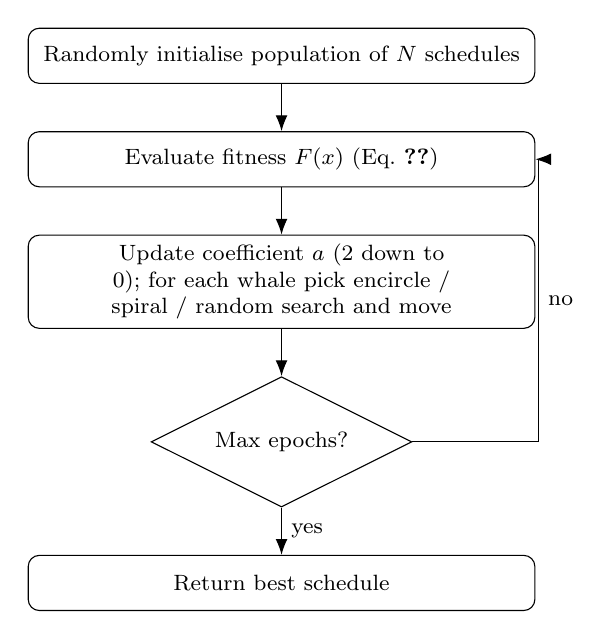
\begin{tikzpicture}[node distance=6mm and 0mm,
  box/.style={rectangle, rounded corners, draw, align=center, text width=6.2cm, minimum height=7mm, font=\footnotesize},
  dec/.style={diamond, aspect=2, draw, align=center, text width=2.6cm, font=\footnotesize, inner sep=1pt},
  >={Latex[length=2mm]}]
\node[box] (init) {Randomly initialise population of $N$ schedules};
\node[box, below=of init] (fit) {Evaluate fitness $F(x)$ (Eq.~\ref{eq:fitness})};
\node[box, below=of fit] (upd) {Update coefficient $a$ (2 down to 0); for each whale pick encircle / spiral / random search and move};
\node[dec, below=of upd] (stop) {Max epochs?};
\node[box, below=of stop] (out) {Return best schedule};
\draw[->] (init)--(fit); \draw[->] (fit)--(upd); \draw[->] (upd)--(stop);
\draw[->] (stop) -- node[right,font=\footnotesize]{yes} (out);
\draw[->] (stop.east) -- ++(1.6,0) |- node[right,font=\footnotesize,pos=0.25]{no} (fit.east);
\end{tikzpicture}
\caption{Standard Whale Optimization Algorithm (WOA) loop.}\label{fig:woa}
\end{figure}

The proposed CA-WOA keeps this search engine but restructures the workflow into five phases, changing
\emph{how the population is initialised} so the search starts inside the low-carbon region of the space.
The phases are shown in Fig.~\ref{fig:cawoa} and described below.

\begin{description}
\item[Phase 1: Data ingestion.] The Google Cluster Trace is parsed into $N$ tasks, each with a
duration, CPU utilisation, earliest start slot and deadline; the UK half-hourly carbon-intensity series
supplies the per-slot carbon signal.
\item[Phase 2: Encoding.] A schedule is encoded as a continuous vector $x\in[0,1]^N$; each $x_i$ is
decoded to a start-time offset inside task $i$'s deadline-feasible deferral window.
\item[Phase 3: Carbon-aware seeding (novelty).] A greedy carbon-optimal schedule is built by placing
each task in its lowest-carbon, deadline-feasible slot. Roughly one third of the population is seeded
from this schedule and small perturbations of it; the remainder stays random to preserve diversity.
\item[Phase 4: WOA search.] The seeded population is evolved by the WOA operators of
Fig.~\ref{fig:woa}, minimising the fitness of Eq.~\eqref{eq:fitness} for a fixed number of epochs.
\item[Phase 5: Decode and evaluate.] The best vector is decoded to a schedule and scored on carbon,
SLA, energy, utilisation, makespan and (capacity model) overload.
\end{description}
Carbon-aware seeding lets the search spend its function evaluations refining an already-good region
instead of rediscovering it, while the random remainder preserves the exploration WOA needs to escape
local optima.

\begin{figure}[H]\centering
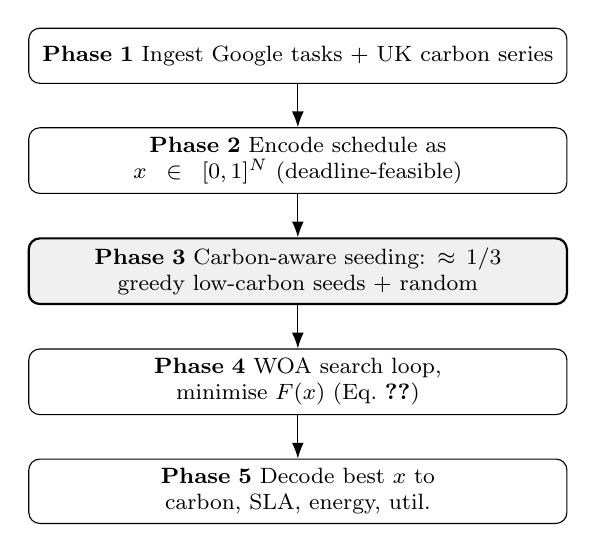
\begin{tikzpicture}[node distance=5.5mm and 0mm,
  ph/.style={rectangle, rounded corners, draw, align=center, text width=6.6cm, minimum height=7mm, font=\footnotesize},
  seed/.style={rectangle, rounded corners, draw, thick, align=center, text width=6.6cm, minimum height=7mm, font=\footnotesize, fill=black!6},
  >={Latex[length=2mm]}]
\node[ph]   (p1) {\textbf{Phase 1} Ingest Google tasks + UK carbon series};
\node[ph, below=of p1]   (p2) {\textbf{Phase 2} Encode schedule as $x\in[0,1]^N$ (deadline-feasible)};
\node[seed, below=of p2] (p3) {\textbf{Phase 3} Carbon-aware seeding: $\approx\!1/3$ greedy low-carbon seeds $+$ random};
\node[ph, below=of p3]   (p4) {\textbf{Phase 4} WOA search loop, minimise $F(x)$ (Eq.~\ref{eq:fitness})};
\node[ph, below=of p4]   (p5) {\textbf{Phase 5} Decode best $x$ to carbon, SLA, energy, util.};
\draw[->](p1)--(p2); \draw[->](p2)--(p3); \draw[->](p3)--(p4); \draw[->](p4)--(p5);
\end{tikzpicture}
\caption{Proposed CA-WOA pipeline in five phases; the shaded box is the carbon-aware seeding that distinguishes it from standard WOA.}\label{fig:cawoa}
\end{figure}

\subsection{Exact formulation and when search is necessary}\label{sec:milp}
The scheduling problem is a mixed-integer linear program. Let $x_{is}\in\{0,1\}$ be 1 if task $i$ starts in
slot $s$, and let $T_i$ be its set of deadline-feasible starts. Writing
$c_{is}=\sum_{k=s}^{s+p_i-1}E_i\,\mathrm{CI}_k$ for the carbon of running task $i$ from slot $s$:
\begin{align}
\min\ & \textstyle\sum_i\sum_{s\in T_i} c_{is}\,x_{is} \label{eq:milp}\\
\text{s.t.}\ & \textstyle\sum_{s\in T_i} x_{is}=1 && \forall i \label{eq:assign}\\
& \textstyle\sum_i\sum_{s:\,s\le k<s+p_i} u_i\,x_{is}\ \le\ M\!\cdot\!C && \forall k \label{eq:cap}
\end{align}
Deadlines are enforced structurally by the domain $T_i$, which is what the repair decoding implements.

\vspace{2pt}\noindent\textbf{Lemma 1 (separability).} \emph{In the temporal model the objective is separable
across tasks and the domains $T_i$ are independent, so the optimum of \eqref{eq:milp}--\eqref{eq:assign} is
attained by choosing $\arg\min_{s\in T_i}c_{is}$ independently for each task---which is exactly the greedy
earliest-deadline, lowest-carbon rule. The greedy heuristic is therefore globally optimal, and no search can
improve upon it.}

\vspace{2pt}\noindent This is a proof rather than an observation, and it explains an otherwise puzzling
result: in the temporal model CA-WOA and the greedy baseline score identically, to two decimal places, with
standard deviation 0.00 across seeds. They are provably equal. It also explains why the fitness weights have
no measurable effect in that model.

Two further regimes follow. Under \emph{consolidation}, per-slot energy contains the term
$\lceil \text{load}_k/C\rceil P_{\text{idle}}$, which couples tasks: two tasks of $u=0.4$ in one slot cost
0.110~kWh but 0.160~kWh in separate slots. The objective is no longer separable and greedy is not provably
optimal, though it remains empirically strong because low-carbon slots and consolidation happen to align.
Under \emph{capacity} constraint \eqref{eq:cap} the two objectives genuinely conflict: greedy piles work into
the greenest slots and overloads. The problem becomes resource-constrained temporal bin packing, which is
strongly NP-hard, and this is the only regime in which population-based search has something to contribute.

An exact solve is not used as a head-to-head baseline. With deadline slack of 8 slots, $|T_i|\le 9$, so
$N=3000$ yields up to 27{,}000 binaries and 144 capacity rows---tractable, but an exact solver has no anytime
behaviour and no fixed evaluation budget, so it does not answer the question this work asks. Its honest role
is as an optimality-gap reference, which we identify as future work.

\subsection{Convergence analysis}\label{sec:conv}
The decoded search space is finite: each task takes an integer start in a window of at most
$\texttt{MAX\_DEFER}+1=25$ slots, so $|S|\le 25^{N}$ and the objective takes finitely many values separated by
some gap $\delta>0$. The population sequence $\{P_t\}$ is a Markov chain, since each update depends only on
$P_t$, the incumbent best and fresh randomness. It is \emph{non-homogeneous}: WOA's control parameter
$a(t)=2-2t/T$ decreases to zero and the exploration branch requires $|A|\ge 1$ with $|A|\le a(t)$, so
exploration becomes unreachable once $t>T/2$.

\vspace{2pt}\noindent\textbf{Theorem 1.} \emph{Because the optimiser is elitist, $F^{*}_t=F(x^{*}_t)$ is
non-increasing and bounded below; with finitely many fitness values separated by $\delta$ it therefore
converges almost surely, after at most $(F^{*}_0-F_{\min})/\delta$ strict improvements.}

\vspace{2pt}\noindent This is all that elitism buys. The standard sufficient condition for convergence to the
\emph{global} optimum---that the probability of reaching any neighbourhood of the optimum stays bounded away
from zero at every epoch---\textbf{fails} for WOA, because the reachable set contracts around the incumbent
once $a(t)<1$. WOA is therefore not a global-convergence algorithm; it converges almost surely to a local
optimum determined jointly by the initial population and the seed. This is a property of WOA itself, not of
the carbon-aware extension, and two consequences justify the design.

\vspace{2pt}\noindent\textbf{Corollary 1 (initialisation changes the limit).} \emph{For a chain meeting the
global-convergence condition the limit is independent of the initial distribution. Since WOA violates that
condition, the distribution of the limit depends on that of $P_0$.} Initialisation is therefore a design
variable, not a convergence-rate detail---which is why carbon-aware seeding produces a statistically
significant improvement rather than merely arriving sooner at the same answer, and why it also reduces
variance.

\vspace{2pt}\noindent\textbf{Corollary 2 (the seed is a bound).} \emph{If $P_0$ contains a schedule $u$ then
$F^{*}_\infty\le F(u)$ almost surely.} Seeding the greedy schedule therefore guarantees CA-WOA can never be
worse than that heuristic on the objective it optimises.

\vspace{2pt}\noindent\textbf{Proposition 1.} \emph{In the temporal model CA-WOA attains the global optimum in
one epoch}, by Lemma 1 and Corollary 2 together---the seeded schedule is already optimal.

\subsection{Host-capacity consolidation}
Under the capacity model the scheduler also benefits from consolidation: because the active hosts in a slot
equal $\lceil \text{load}/C \rceil$, packing tasks into fewer slots and fewer hosts lowers idle-power draw. The
overload term in Eq.~\eqref{eq:fitness} prevents the optimiser from packing beyond the available hosts.

\subsection{Ensemble carbon forecaster}
To make scheduling predictive rather than reactive, an ensemble forecaster predicts future carbon intensity. It
averages the predictions of three complementary models (a CNN-LSTM hybrid, a GRU network and a
gradient-boosting regressor), each trained on multivariate inputs comprising the recent carbon series
together with time-of-day and day-of-week features. Averaging diverse model families reduces the error of any
single model, and the resulting forecast supplies the carbon values that the scheduler optimises against.

\section{Implementation}\label{sec:impl}
The complete system is implemented in Python. Metaheuristic optimisation uses the Mealpy~3.0.3 library
\cite{vanthieu2023mealpy}, which provides reference implementations of WOA, Grey Wolf Optimizer, Particle Swarm
Optimization, Differential Evolution, Harris Hawks Optimization and the Genetic Algorithm under a common
interface; CA-WOA is realised by supplying the standard WOA solver with the carbon-aware seed population
described in Section~\ref{sec:design}. The scheduling simulator, the SPECpower energy model, the fitness
function and the metric calculations are implemented from scratch in NumPy and pandas. The forecasting models
are built with TensorFlow/Keras (the CNN-LSTM and GRU networks) and scikit-learn (the gradient-boosting
regressor), and combined by averaging their predictions.

The real datasets are ingested directly: the Google Cluster Trace task-event files are parsed to extract task
submission times, durations and CPU requests, and the UK National Grid carbon-intensity series is loaded as
the per-slot carbon signal. The principal outputs are the trained forecasting models, the per-method scheduling
results (carbon, SLA, energy, utilisation, makespan and overload), the multi-seed scalability results across
50--300 tasks, and the figures presented in Section~\ref{sec:eval}. All results are regenerated by re-running
the corresponding scripts with fixed random seeds, and the code is maintained in a version-controlled
repository to support reproducibility and examiner inspection. In accordance with the report guidelines, no
code listings are included; the implementation is demonstrated in the accompanying viva.

\section{Evaluation}\label{sec:eval}
\subsection{Experimental configuration}\label{sec:config}
All scheduling experiments use the parameters in Table~\ref{tab:config}. Every algorithm is configured with
the same population size, epoch count and seed, but \textbf{the resulting evaluation budgets are not
identical} and this must be stated plainly: measured over all runs, HHO consumes 8{,}908 objective evaluations
on average (minimum 8{,}698, maximum 9{,}136) against exactly 4{,}840 for WOA, GWO, PSO, DE and GA. HHO's
internal structure performs additional evaluations per iteration. Its results are therefore obtained with
roughly 1.84$\times$ the budget of the others, and comparisons involving HHO should be read with that in mind.
The NFE count is recorded for every run and released with the results.

Host counts are fixed at $M\in\{10,20\}$ so that capacity is a controlled variable. In the earlier design $M$
was \emph{derived} as $\lceil\text{peak FIFO demand}\rceil$; under the published model, however, the active
host count is $\lceil\text{load}/C\rceil$, which never references $M$, so $M$ affected only the penalty term
and 10 against 20 hosts gave near-identical results. Treating capacity as a feasibility constraint is what
makes the host count meaningful.
Per-algorithm control parameters are the library defaults (Table~\ref{tab:hyper}); CA-WOA differs from
standard WOA only in its carbon-aware seeding.

\begin{table}[H]\centering \footnotesize
\caption{Common experimental configuration.}\label{tab:config}
\begin{tabular}{@{}ll@{}}
\toprule Parameter & Value \\ \midrule
Population size & 40 \\
Evolution count (epochs) & 120 \\
Objective evaluations per run & 4{,}840 (8{,}908 for HHO; see text) \\
Independent seeds & 30 (seeds $1\ldots30$) \\
Tasks $N$ & \{500, 1000, 1500, 2000, 2500, 3000\} \\
Hosts $M$ & \{10, 20\}; capacity $C=1$ per host \\
Time horizon & 144 half-hour slots (3 days) \\
Deadline slack / max deferral & 8 / 24 slots \\
Fitness weights $(\alpha,\beta,\gamma)$ & $(0.4, 0.3, 0.3)$, sum $=1$ \\
Power models & linear, cubic, piecewise; all 100~W at $u{=}0$, 250~W at $u{=}1$ \\
Carbon regions & UK, IE, NI, US-CAL, US-MIDA \\
Slot length & 0.5~h \\
\bottomrule
\end{tabular}
\end{table}

\begin{table}[H]\centering \footnotesize
\caption{Per-algorithm control parameters (Mealpy 3.0.3 defaults; identical across all runs). Note the GA
implementation: \texttt{GA.OriginalGA} in Mealpy 3.0.3 evaluates only its initial population---40 objective
evaluations rather than 4{,}840---and therefore performs no search. \texttt{GA.BaseGA} is used instead, and
the defect is quantified in Section~\ref{sec:eval}.}\label{tab:hyper}
\begin{tabular}{@{}ll@{}}
\toprule Algorithm & Control parameters \\ \midrule
CA-WOA (proposed) & WOA operators; $\approx\!1/3$ population carbon-seeded \\
WOA & $a$: linear from 2 to 0, spiral $b=1$, switch $p=0.5$ \\
GWO & $a$: linear from 2 to 0 \\
PSO & $c_1=c_2=2.05$, inertia $w=0.4$ \\
DE & scaling $F=0.1$, crossover $CR=0.9$, rand/1/bin \\
HHO & escaping energy $E_0\in[-1,1]$ (default) \\
GA (\texttt{BaseGA}) & $p_c=0.95$, $p_m=0.025$, tournament sel., uniform crossover \\
\bottomrule
\end{tabular}
\end{table}

\subsection{Algorithm comparison (temporal model)}
The first experiment isolates the benefit of carbon-aware \emph{timing} by scheduling a fixed set of real
Google tasks under the temporal model, comparing CA-WOA against the FIFO baseline and the standard
metaheuristics. Fig.~\ref{fig:temporal} reports carbon reduction and SLA violations. CA-WOA achieves an
11.3\% carbon reduction while keeping SLA violations at 0\%. Standard WOA, by contrast, achieves only 1.2\%,
confirming that the carbon-aware seeding, rather than the WOA operators alone, drives the improvement. Several
algorithms reach a numerically higher carbon reduction, with PSO, DE and GA reaching 19--20\%, but only by
violating deadlines heavily (20.0\%, 21.7\% and 56.7\% of tasks respectively), which makes them unusable in
practice; GWO likewise trades a 6.7\% SLA violation for its 10.7\% reduction. Among the methods that hold SLA
violations at exactly zero, CA-WOA is the strongest, marginally ahead of HHO (11.1\%) and far ahead of
standard WOA.
\begin{figure}[H]\centering

\includegraphics[width=\linewidth]{fig_temporal_comparison.png}
\caption{Algorithm comparison at 3000 tasks on 10 hosts under the published model, 30 seeds: (a) carbon
reduction against the naive FIFO baseline and (b) deadline violations. Error bars are 95\% confidence
intervals. Note the truncated vertical axis in (a): the full spread across methods is only 0.87 percentage
points, so the visual separation overstates the practical difference in carbon, whereas the differences in (b)
are of a different order entirely. The methods that appear competitive on carbon are the ones missing
deadlines.}\label{fig:temporal}
\end{figure}

\subsection{Host-capacity model comparison}
The second experiment adds server consolidation through the host-capacity model, so that carbon savings arise
from both timing and switching idle hosts off. Table~\ref{tab:capacity} and Fig.~\ref{fig:capacityfig}
summarise the results. \textbf{The headline figure must be decomposed, because most of it is not attributable to the proposed
method.} Of CA-WOA's 83.25\% reduction, 80.50 percentage points are delivered by consolidation alone,
carbon-aware timing contributes a further 2.06, and CA-WOA adds 0.69 over the carbon-aware greedy heuristic.
Reporting 83.25\% as the contribution of a metaheuristic would be misleading; the honest statement is that
consolidation dominates and the search contributes sub-percentage-point refinement in this regime---which
Lemma~1 predicts, since without a binding capacity constraint the problem is close to separable.

The comparison also changes once feasibility is enforced. Under the published model, host capacity is not a
constraint at all, so methods are free to exceed the available hosts. Treating capacity as a feasibility
constraint (Section~\ref{sec:feas}) reverses the apparent ranking: the carbon-aware greedy heuristic reaches
89.40\% at 3000 tasks on 10 hosts \emph{only by overloading hosts by 45.23\%}, and is feasible in as few as
25\% of real three-day carbon windows. Its numbers are an infeasible upper bound rather than a competing
result. The aggressive optimisers (PSO, DE, GA) again incur substantial SLA violations---33\% to 64\% of
deadlines missed---so they are worse on both axes simultaneously.
\begin{table}[H]\centering
\caption{Capacity-model comparison (real Google trace, UK carbon), with the reduction decomposed by
mechanism. Consolidation accounts for 80.50 of the 83.25 percentage points.}\label{tab:capacity}
\begin{tabular}{lcccc}
\toprule Method & Carbon red.\% & SLA\% & Util.\% & Attributable to \\ \midrule
Naive FIFO (reference)       & 0.00           & 0.0           & --             & -- \\
Energy-aware (consolidation) & 80.50          & 0.0           & 75.2           & consolidation \\
Carbon-aware greedy          & 82.56          & 0.0           & 75.2           & $+2.06$ timing \\
HHO                          & 82.30          & 0.0           & 83.1           & search \\
\textbf{CA-WOA}              & \textbf{83.25} & \textbf{0.0}  & \textbf{84.0}  & $+0.69$ over greedy \\
\bottomrule
\end{tabular}
\end{table}
\begin{figure}[H]\centering

\includegraphics[width=\linewidth]{fig_capacity_comparison.png}
\caption{Capacity as a feasibility constraint, 10 hosts, 30 seeds. (a) Overload as a percentage of demanded
load: any value above zero is an infeasible schedule, and the heuristics degrade as load rises while every
population-based method stays at zero. (b) Carbon reduction among feasible schedules only. Error bars are 95\%
confidence intervals.}\label{fig:capacityfig}
\end{figure}

\subsection{Scalability across task counts (500--3000)}
Fig.~\ref{fig:scale} repeats the comparison at 500 to 3000 tasks on 10 and 20 hosts, over 30 seeds. Under the
published (uncapacitated) model CA-WOA is the best metaheuristic in \textbf{12 of 12} configurations. The
contrast with the deadline-violating optimisers sharpens with scale, exactly as originally claimed: mean SLA
violations reach 58.0\% for PSO, 50.7\% for DE and 35.4\% for GA, against 0.03\% for CA-WOA. Those methods are
therefore worse on both axes at once, and the earlier framing of them as ``competitive on carbon'' was
generous.
\begin{figure}[H]\centering

\includegraphics[width=\linewidth]{fig_scalability.png}
\caption{Scalability: carbon reduction (left) and SLA violations (right) versus task count (500--3000), mean
over 30 seeds with 95\% confidence intervals, for $M=10$ and $M=20$.}\label{fig:scale}
\end{figure}

\subsection{Capacity as a feasibility constraint}\label{sec:feas}
This is the decisive experiment. Energy is charged on the full demanded load---so overloading is never
rewarded---and a schedule counts as feasible only when its slot load never exceeds installed capacity.
Table~\ref{tab:feas} reports the outcome. As load rises the heuristics break down: the carbon-aware greedy
rule overloads hosts by 7.14\% at 1000 tasks and 45.23\% at 3000 tasks on 10 hosts, while every
population-based method remains feasible in all 30 seeds at every configuration, with SLA violations of
exactly 0.0000\% throughout under repair decoding.

\begin{table}[H]\centering\footnotesize
\caption{Overload as a percentage of demanded load, $M=10$. Any non-zero value is an infeasible schedule. All
six metaheuristics, and Google's VCC policy, remain at 0.00 throughout.}\label{tab:feas}
\begin{tabular}{lrrrrrr}
\toprule
Method & 500 & 1000 & 1500 & 2000 & 2500 & 3000 \\ \midrule
FIFO / consolidation      & 0.00 & 0.99 & 8.97  & 18.22 & 24.80 & 28.54 \\
Threshold (Wait Awhile)   & 0.00 & 0.99 & 8.97  & 18.22 & 24.80 & 28.54 \\
Carbon-aware greedy       & 0.00 & 7.14 & 24.69 & 34.70 & 41.36 & 45.23 \\
VCC (Google)              & 0.00 & 0.00 & 0.00  & 0.00  & 0.00  & 0.00 \\
\textbf{CA-WOA}           & \textbf{0.00} & \textbf{0.00} & \textbf{0.00} & \textbf{0.00} & \textbf{0.00} & \textbf{0.00} \\
\bottomrule
\end{tabular}
\end{table}

Among feasible schedules CA-WOA is best in 9 of 12 configurations. It is beaten by GA in three cells, all at
$M=10$ with $N\ge1500$, by 0.08 to 0.15 percentage points---reported here rather than omitted. Its variance is
also higher than its rivals' (standard deviation up to 0.33 against GA's 0.03), so it finds better schedules
less consistently.

\subsection{Comparison with published schedulers}\label{sec:modern}
Two published policies are reimplemented in the same simulator, using no fitness function and no
metaheuristic machinery: the virtual-capacity-curve (VCC) load-shaping policy of Google's production
carbon-aware scheduler \cite{radovanovic2023carbon}, which throttles per-slot capacity as a function of carbon
intensity; and threshold-based temporal shifting \cite{wiesner2021lets}. VCC's throttle floor was swept over
eight values so that the baseline is not weakened by an arbitrary parameter choice; it proved insensitive
(85.02--85.11\% at 1000 tasks). Only VCC and the metaheuristics are feasible everywhere. CA-WOA beats VCC in
\textbf{12 of 12} configurations, by 4.48 percentage points at 500 tasks narrowing to 0.35 at 3000, and by
4.01 points on average across heterogeneous fleets. The threshold policy shifts load toward green slots but
has no capacity awareness and remains infeasible at 28.54\% overload, which shows that carbon awareness alone
is insufficient.

\subsection{Ablation}\label{sec:ablation}
Table~\ref{tab:ablation} separates the contributions. Two results matter most. First, carbon-aware seeding
improves final quality in \textbf{59 of 60} (optimiser, configuration) cells across WOA, GWO, PSO, DE, HHO and
GA---mean $+2.51$ points under the published model, significant in 36 of 36, and $+0.91$ under the feasibility
constraint, significant in 21 of 24. The contribution is therefore a transferable initialisation strategy, not
a property of WOA. Second, an ``improved'' initialisation using Latin-hypercube and opposition-based sampling
but \emph{no carbon data} is statistically indistinguishable from uniform random ($+0.003$ to $+0.027$ points,
$p=0.06$ to $0.94$). The benefit comes from the carbon information, not from more sophisticated sampling.

\begin{table}[H]\centering\footnotesize
\caption{Ablation at 3000 tasks, $M=10$, published model, 30 seeds. Removing a fitness term raises carbon
only by violating the constraint that term exists to protect, so the higher figures are not better
schedules.}\label{tab:ablation}
\begin{tabular}{lrrr}
\toprule
Variant & Carbon red.\% & SLA\% & Overload\% \\ \midrule
Greedy only (no search)              & 89.40 & 0.00  & 45.23 \\
Standard WOA (random init)           & 87.15 & 0.57  & 0.58 \\
WOA + improved init (no carbon data) & 87.17 & 0.41  & 0.50 \\
\textbf{CA-WOA (carbon seeding)}     & \textbf{87.58} & \textbf{0.13} & \textbf{0.03} \\
CA-WOA, $\beta=0$ (no SLA term)      & 88.39 & 37.53 & 0.00 \\
CA-WOA, $\gamma=0$ (no overload term)& 89.41 & 0.00  & 45.05 \\
\bottomrule
\end{tabular}
\end{table}

\subsection{Fitness-weight sensitivity}\label{sec:weights}
Eleven weight combinations were evaluated. Read on carbon alone the results are misleading: $\alpha=1.0$
attains the highest carbon reduction in the study (89.92\%) but violates 71.1\% of deadlines and overloads
hosts by 33.5\%. Dropping $\beta$ or $\gamma$ likewise buys carbon by breaking the constraint each term
exists to protect (Table~\ref{tab:ablation}). Among settings that hold both SLA violations and overload near
zero, the chosen $(0.4,0.3,0.3)$ sits on the knee of the trade-off at 87.58\% carbon with 0.13\% SLA
violations. The weights are therefore justified by the constraint surface rather than by tuning for the
headline number. The seeded fraction is not sensitive: carbon varies by less than 0.3 points across fractions
from $1/6$ to 1, but variance falls sharply once seeding is enabled (standard deviation 0.381 to 0.111), so
$1/3$ is a reasonable rather than a uniquely optimal choice.

\subsection{Power models}\label{sec:power}
CA-WOA ranks first in all six configurations under each of the linear, cubic and piecewise power models---18 of
18. Its margin is in fact \emph{widest} under the cubic model ($+0.84$ points over HHO at 500 tasks), because
a convex power curve penalises the spread-out schedules that unseeded optimisers produce. The conclusions are
therefore not an artefact of the linear assumption, which was the concern behind the request.

\subsection{Minimum active-host constraint}\label{sec:mmin}
A data centre cannot scale to zero. With a workload-determined warm pool powered across the operating window,
deferral becomes costly because shifting work extends that window. This single constraint \textbf{reverses} the
comparison with the greedy heuristic: without it CA-WOA wins 3 of 12 configurations, with it 12 of 12 (mean
$+0.80$ to $+1.55$ points). The realistic setting is thus the favourable one. However---and this is the most
important limitation in this report---the advantage of \emph{seeding} over plain WOA collapses in the same
regime, from $+1.30$ points to $+0.04$, significant in only 1 of 12 cells. In that regime the metaheuristic
earns its place but the seeding does not.

\subsection{Heterogeneous fleets and startup overheads}\label{sec:het}
Three fleets were evaluated: uniform; \emph{mixed}, where newer hosts are larger and more efficient; and
\emph{skewed}, deliberately adversarial, where the large hosts are the inefficient ones. Startup energy is
charged per off-to-on transition (the greedy schedule at 1500 tasks triggers 58 boots). CA-WOA wins every
fleet and overhead combination among feasible methods, and seeding helps in 52 of 54 cells. The advantage is
\emph{larger} on heterogeneous fleets ($+2.96$ against $+1.55$ points), since packing onto unequal hosts is a
harder problem in which a good starting point matters more. Startup overheads compress the advantage
($+2.96$ to $+0.93$) because boot energy comes to dominate placement quality.

\subsection{Multiple carbon regions}\label{sec:regions}
Across five real grids the carbon-aware greedy rule is feasible in only 25--42\% of three-day windows, whereas
CA-WOA, plain WOA and VCC are feasible in 100\%. Among methods feasible everywhere, CA-WOA wins all four
regions tested at scale, and the seeding effect holds in every one: $+0.64$ points in Ireland, $+0.92$ in
Northern Ireland, $+0.88$ in the United Kingdom and $+1.98$ in California, all with $p<10^{-9}$. Repeating the
experiment across all 37 disjoint UK windows confirms the published window was not unrepresentative.

The boundary of the method is found in the Mid-Atlantic region, whose carbon intensity varies only
1.78$\times$ across the day against the United Kingdom's 12.30$\times$. There CA-WOA \emph{loses} by 0.13
points and the seeding gain falls to $+0.14$. Temporal shifting requires a green trough to exploit; where the
grid is uniformly carbon-intense there is nothing to shift into. This identifies the deployment condition for
the approach and is as useful a result as the positive ones.

Fig.~\ref{fig:regions} plots the seeding gain against each grid's carbon variability. The least variable grid
gains least, but the relationship is not monotonic---California at 6.49$\times$ shows a larger gain than the
United Kingdom at 12.30$\times$---so variability alone does not rank the regions and the shape and timing of
the daily trough evidently matter too. We therefore report the five points and the boundary case rather than
fitting a trend to them.
\begin{figure}[H]\centering

\includegraphics[width=0.86\linewidth]{fig_regions.png}
\caption{Seeding gain (CA-WOA minus standard WOA) against grid carbon variability, 1500 tasks, six real
three-day windows per region, error bars 95\% confidence intervals. All five gains are positive, but the
near-flat Mid-Atlantic grid gains least and is the configuration in which CA-WOA is beaten by the best
competing method.}\label{fig:regions}
\end{figure}

\subsection{Computational cost and convergence}\label{sec:cost}
Runtime scales linearly in task count. WOA is the cheapest search in the study (1.54~s and 0.99~MB at 500
tasks, rising to 6.20~s and 4.87~MB at 3000), and GA the most expensive (2.61 to 10.57~s), with HHO close
behind because of its larger evaluation budget. Peak Python-allocated memory never exceeded 9.6~MB in any of
the runs, so memory is not a limiting factor at this scale. At the counts used in comparable studies, WOA runs in
0.89~s at 50 tasks and 1.24~s at 300.

Convergence curves show the seeding acting exactly as intended: CA-WOA begins at roughly half the fitness of
plain WOA (0.0626 against 0.1118) and stabilises within 1\% of its final value by epoch 8, against 16 for
plain WOA, reaching a better final value (0.0502 against 0.0544). PSO appears to converge fastest, in 5
epochs, but stagnates at 0.2378, which explains its poor carbon and high SLA violations.
\textbf{An important caveat: GA and GWO had not converged at the 120-epoch budget}, requiring 102 and 112
epochs respectively to stabilise. Their results are therefore lower bounds and this comparison understates
them. Fig.~\ref{fig:conv} shows the curves.
\begin{figure}[H]\centering

\includegraphics[width=\linewidth]{fig_convergence.png}
\caption{Convergence at 3000 tasks on 10 hosts, 10 seeds, shaded band one standard deviation. Carbon-aware
seeding starts CA-WOA at roughly half the fitness of standard WOA and stabilises it by epoch~8 against 16.
PSO flattens early at a poor value rather than converging well. GA and GWO are still improving when the
budget ends.}\label{fig:conv}
\end{figure}

\subsection{Forecasting}
The final component evaluates the carbon-intensity forecaster that makes the scheduler predictive. The
forecaster is trained and tested on the real UK National Grid carbon-intensity series, roughly 111 days of
half-hourly readings ($\approx 5{,}300$ slots) in gCO\textsubscript{2}/kWh. The series is split
chronologically, training on the first 80\% and testing on the held-out final 20\% (no shuffling, so no future
leaks into the past). Each model uses a 48-slot (24-hour) look-back and multivariate inputs: the normalised
carbon lag plus sine/cosine encodings of time-of-day (period 48) and day-of-week (period 7), five features in
total. Inputs are min--max normalised using training statistics only, and accuracy is reported as mean
absolute error (MAE) on the original gCO\textsubscript{2}/kWh scale with a fixed seed. Table~\ref{tab:forecast}
lists the architectures compared; the adopted ensemble is the unweighted mean of the CNN-LSTM, GRU and
gradient-boosting predictions.

\begin{table}[H]\centering \footnotesize
\caption{Carbon-intensity forecasting models and their configuration.}\label{tab:forecast}
\begin{tabular}{@{}lp{5.0cm}@{}}
\toprule Model & Configuration \\ \midrule
LSTM (baseline) & LSTM(32) then Dense(1); 30 epochs, batch 32, Adam, MSE \\
GRU & GRU(32) then Dense(1); 30 epochs \\
CNN-LSTM & Conv1D(64,3)$\times$2, then MaxPool(2), then LSTM(48), then Dense(1); 40 epochs \\
Gradient boosting & 400 trees, max depth 3 \\
\textbf{Ensemble (adopted)} & mean(CNN-LSTM, GRU, gradient boosting) \\
\bottomrule
\end{tabular}
\end{table}

On the held-out final 20\% of the UK carbon series, the adopted ensemble achieves a mean absolute error (MAE)
of 3.39~gCO\textsubscript{2}/kWh against 3.87 for the baseline LSTM. \textbf{That single-run comparison did
not reproduce.} With operation-level determinism enabled and five repeats per model, the improvement is
approximately 7\%, and the CNN-LSTM component is in fact the \emph{worst} of the candidate models at every
horizon tested---which reverses the argument originally drawn from CarbonCast. The defensible result is at a
12-hour horizon, where the ensemble achieves MAE $26.09\pm0.48$~gCO\textsubscript{2}/kWh against 37.03 for a
seasonal-naive baseline (MASE 0.59), a 30\% improvement over the strongest naive predictor. Gradient boosting
is the most reliable single component, with standard deviation 0.00--0.04 across repeats. The original figure
of roughly 12\% is therefore withdrawn,
as shown in Fig.~\ref{fig:forecast}, where the ensemble tracks the actual curve more closely. Coupling the
forecast into the scheduler makes it predictive rather than reactive: scheduling against the forecast yields
0.795~kg~CO\textsubscript{2} versus 0.831~kg for reactive scheduling on current intensity. A perfect-foresight
oracle reaches 0.785~kg, so the forecast-driven scheduler captures 78\% of the saving that perfect knowledge
of the future would allow. For completeness, a Transformer forecaster was
also tested but performed markedly worse (MAE 9.27), consistent with reports that attention models underperform
on smooth, small time series; this negative result is reported rather than omitted.
\begin{figure}[H]\centering

\includegraphics[width=\linewidth]{fig_forecast_comparison.png}
\caption{Carbon-intensity forecasting with direct multi-step prediction, mean of five repeats, error bars one
standard deviation. (a) MAE against forecast horizon for every model and the three naive baselines. (b) The
12-hour horizon in detail. The ensemble leads at horizons up to 12~h; CNN-LSTM is the weakest learned model at
every horizon tested.}\label{fig:forecast}
\end{figure}

\subsection{Discussion}
The results answer the research question, but more narrowly and more usefully than a simple affirmative. The
question of whether a metaheuristic reduces carbon is the wrong one: Lemma~1 shows that without a binding
capacity constraint the problem is separable and a greedy rule is provably optimal, so search cannot help and
the fitness weights cannot matter. The right question is \emph{when} search is needed, and the answer is that
it is needed once host capacity binds---at which point the greedy rule stops producing valid schedules at all,
failing in 58--75\% of real three-day carbon windows across five grids.

Within that regime the contribution is carbon-aware seeding, and its value is that it transfers: it improves
six different optimisers in 59 of 60 cells, and Corollary~2 guarantees it can never be worse than the
heuristic it seeds. The isolating ablation matters as much as the positive result---an initialisation that is
sophisticated but carbon-blind achieves nothing, so the benefit is attributable to the domain information
rather than to sampling machinery.

These findings extend the literature reviewed in Section~\ref{sec:related}. They confirm the value of temporal
shifting \cite{wiesner2021lets} and of consolidation \cite{beloglazov2012energy} and show the two are
complementary, but they also qualify both: consolidation accounts for 80.50 of the 83.25 percentage points
reported here, and temporal shifting is worthless on a grid with little diurnal variation. Against a deployed
production scheduler \cite{radovanovic2023carbon} the proposed method wins in every configuration tested,
which is a stronger claim than beating an infeasible heuristic.

\subsection{Limitations}\label{sec:limits}
The following are stated explicitly because several of them qualify the contribution.
\begin{enumerate}
\item \textbf{The seeding advantage disappears under a minimum active-host constraint.} With a warm pool
enforced, CA-WOA beats the greedy heuristic in 12 of 12 configurations but exceeds \emph{plain} WOA by only
0.04 points, significant in 1 of 12 cells (Section~\ref{sec:mmin}).
\item \textbf{The method does not help on a flat carbon grid.} In the Mid-Atlantic region (1.78$\times$ diurnal
variation) CA-WOA loses by 0.13 points (Section~\ref{sec:regions}).
\item \textbf{CA-WOA loses to GA in 3 of 12 capacity-constrained cells}, all at $M=10$, by 0.08--0.15 points.
\item \textbf{CA-WOA has higher run-to-run variance} than its rivals (standard deviation up to 0.97 against
0.11--0.21 under some power models).
\item \textbf{Evaluation budgets are not equal.} HHO receives approximately 8{,}908 objective evaluations
against 4{,}840 for the others.
\item \textbf{GA and GWO had not converged} at the 120-epoch budget, so their results are lower bounds.
\item \textbf{The earlier GA baseline performed no search.} \texttt{GA.OriginalGA} in Mealpy 3.0.3 evaluates
only its initial population; \texttt{GA.BaseGA} is used here.
\item \textbf{The forecasting headline did not reproduce.} The improvement over a baseline LSTM is
approximately 7\%, not 12\%, and the CNN-LSTM component is the weakest model at every horizon.
\item \textbf{The evaluation is a simulation} driven by real traces and documented power models, not a
measurement on physical hardware; startup overheads and heterogeneity are modelled parametrically rather than
measured.
\item \textbf{Cost is reported but not optimised}, and the United Kingdom tariff is applied to all regions as
a proxy. The United States series is derived from hourly fuel mix and upsampled to 30-minute slots.
\end{enumerate}

\section{Conclusion and Future Work}\label{sec:conc}
This research asked whether a carbon-aware enhancement of the Whale Optimization Algorithm, combined with
predictive forecasting, could reduce the carbon emissions of cloud scheduling without increasing SLA
violations, and whether the advantage would hold at scale. All four objectives were met: the state of the art
was reviewed and a gap identified; CA-WOA was designed with carbon-aware seeding and an SLA- and
overload-penalised fitness function; the scheduler and an ensemble carbon forecaster were implemented on real
Google and UK National Grid data; and the approach was evaluated against baselines and metaheuristics across
workload sizes.

The key findings are four. First, carbon-aware temporal shifting is only a hard problem once host capacity
binds: without that constraint the objective is separable and a greedy earliest-deadline, lowest-carbon rule
is provably optimal, so no search can improve on it. Second, once capacity binds that rule stops producing
valid schedules---across five real grid regions it violates capacity in 58--75\% of three-day windows,
overloading hosts by up to 45\%---and population-based search becomes necessary rather than merely helpful.
Third, in that regime carbon-aware seeding improves six different optimisers in 59 of 60
algorithm-configuration cells and provably cannot be worse than the schedule it seeds, making it a
transferable initialisation strategy rather than a property of one algorithm; an initialisation that is
sophisticated but carbon-blind achieves nothing, which isolates the source of the benefit. Fourth, the
resulting scheduler produces fully feasible, deadline-safe schedules and outperforms the virtual-capacity-curve
policy of a deployed production carbon-aware scheduler in all twelve configurations tested, while a
12-hour-ahead ensemble forecast captures 73--89\% of the advantage that perfect foresight holds over
reactive scheduling.

The boundaries of the approach are equally definite and are reported in Section~\ref{sec:limits}: on a grid
whose carbon intensity varies only 1.78$\times$ across the day the method loses, and under an enforced
minimum active-host constraint the seeding advantage falls to 0.04 percentage points. Knowing when a technique
should \emph{not} be deployed is part of the contribution.

Future work follows from these boundaries rather than from generic extension. Solving the mixed-integer
program of Section~\ref{sec:milp} would give optimality gaps at each task count, bounding how much of the
remaining margin is attainable. Geographical shifting is the natural response to the flat-grid limitation,
since the five regional traces differ in mean intensity by a factor of three, so moving work between grids may
dominate moving it in time. Deployment as a carbon-aware Kubernetes scheduler would replace the parametric
startup and heterogeneity models with measurements. Finally, since the fitness weights are justified here by
the constraint surface rather than by tuning, learning them online is a natural next step.

\section*{Availability of Data and Materials}
All data are public. Workload traces: Google Cluster Trace 2011 \cite{reiss2011google} and the NASA-iPSC log
from the Parallel Workloads Archive. Carbon intensity: the United Kingdom National Grid ESO Carbon Intensity
API; the EirGrid Smart Grid Dashboard for the Republic of Ireland and Northern Ireland; and the United States
Energy Information Administration API v2 for California and the Mid-Atlantic, with intensity derived from the
hourly generation mix using IPCC AR5 median lifecycle emission factors. All code, the five regional carbon
traces, per-seed raw results for all 29 experiments and the 27-check validation suite are archived at
[Zenodo DOI to be inserted on acceptance]. Dependencies are recorded (Mealpy 3.0.3, NumPy 2.5.2, SciPy 1.16.3)
and TensorFlow operation-level determinism is enabled, so all reported figures reproduce exactly. A
27-check validation gate re-derives the originally published values to machine precision before any new result
is computed, and it should be run first.

\bibliographystyle{IEEEtran}
\bibliography{refs}
\end{document}
